\documentclass[12pt, oneside]{article}

\usepackage[letterpaper, scale=0.89, centering]{geometry}
\usepackage{fancyhdr}
\setlength{\parindent}{0em}
\setlength{\parskip}{1em}

\pagestyle{fancy}
\fancyhf{}
\renewcommand{\headrulewidth}{0pt}
\rfoot{\href{https://creativecommons.org/licenses/by-nc-sa/2.0/}{CC BY-NC-SA 2.0} Version \today~(\thepage)}

\usepackage{amssymb,amsmath,pifont,amsfonts,comment,enumerate,enumitem}
\usepackage{currfile,xstring,hyperref,tabularx,graphicx,wasysym}
\usepackage[labelformat=empty]{caption}
\usepackage[dvipsnames,table]{xcolor}
\usepackage{multicol,multirow,array,listings,tabularx,lastpage,textcomp,booktabs}

\lstnewenvironment{algorithm}[1][] {   
    \lstset{ mathescape=true,
        frame=tB,
        numbers=left, 
        numberstyle=\tiny,
        basicstyle=\rmfamily\scriptsize, 
        keywordstyle=\color{black}\bfseries,
        keywords={,procedure, div, for, to, input, output, return, datatype, function, in, if, else, foreach, while, begin, end, }
        numbers=left,
        xleftmargin=.04\textwidth,
        #1
    }
}
{}
\lstnewenvironment{java}[1][]
{   
    \lstset{
        language=java,
        mathescape=true,
        frame=tB,
        numbers=left, 
        numberstyle=\tiny,
        basicstyle=\ttfamily\scriptsize, 
        keywordstyle=\color{black}\bfseries,
        keywords={, int, double, for, return, if, else, while, }
        numbers=left,
        xleftmargin=.04\textwidth,
        #1
    }
}
{}

\newcommand\abs[1]{\lvert~#1~\rvert}
\newcommand{\st}{\mid}

\newcommand{\A}[0]{\texttt{A}}
\newcommand{\C}[0]{\texttt{C}}
\newcommand{\G}[0]{\texttt{G}}
\newcommand{\U}[0]{\texttt{U}}

\newcommand{\cmark}{\ding{51}}
\newcommand{\xmark}{\ding{55}}

 
\begin{document}
\begin{flushright}
    \StrBefore{\currfilename}{.}
\end{flushright} 
\section*{Monday November 1}

Today's session is on Zoom, log in with your @ucsd.edu account https://ucsd.zoom.us/j/97431852722
Meeting ID: 974 3185 2722



{\it Recall the definitions}: The set of RNA strands $S$ is defined (recursively) by:
\[
\begin{array}{ll}
\textrm{Basis Step: } & \A \in S, \C \in S, \U \in S, \G \in S \\
\textrm{Recursive Step: } & \textrm{If } s \in S\textrm{ and }b \in B \textrm{, then }sb \in S
\end{array}
\]
where $sb$ is string concatenation.

The function \textit{rnalen} that computes the length of RNA strands in $S$ is defined recursively by:
\[
\begin{array}{llll}
& & \textit{rnalen} : S & \to \mathbb{Z}^+ \\
\textrm{Basis Step:} & \textrm{If } b \in B\textrm{ then } & \textit{rnalen}(b) & = 1 \\
\textrm{Recursive Step:} & \textrm{If } s \in S\textrm{ and }b \in B\textrm{, then  } & \textit{rnalen}(sb) & = 1 + \textit{rnalen}(s)
\end{array}
\]

The function \textit{basecount} that computes the number of a given base 
$b$ appearing in a RNA strand $s$ is defined recursively by:
\[
\begin{array}{llll}
& & \textit{basecount} : S \times B & \to \mathbb{N} \\
\textrm{Basis Step:} &  \textrm{If } b_1 \in B, b_2 \in B & \textit{basecount}(~(b_1, b_2)~) & =
        \begin{cases}
            1 & \textrm{when } b_1 = b_2 \\
            0 & \textrm{when } b_1 \neq b_2 \\
        \end{cases} \\
\textrm{Recursive Step:} & \textrm{If } s \in S, b_1 \in B, b_2 \in B &\textit{basecount}(~(s b_1, b_2)~) & =
        \begin{cases}
            1 + \textit{basecount}(~(s, b_2)~) & \textrm{when } b_1 = b_2 \\
            \textit{basecount}(~(s, b_2)~) & \textrm{when } b_1 \neq b_2 \\
        \end{cases}
\end{array}
\] 
At this point, we've seen the proof strategies
\begin{multicols}{2}
    \begin{itemize}
        \item A {\bf counterexample} to prove that  $\forall x P(x)$ is {\bf false}.
        \item  A {\bf witness} to prove that  $\exists x P(x)$ is {\bf true}.
        \item {\bf Proof of universal by exhaustion} to prove that $\forall x \, P(x)$
    is true when $P$ has a finite domain
        \item  {\bf Proof by universal generalization} to prove that $\forall x \, P(x)$
    is true using an arbitrary element of the domain.
        \item To  prove  that $\exists x P(x)$ is {\bf false}, write the universal statement that is 
        logically equivalent to its negation and then prove it true using universal generalization.
        \item To prove that $p \land q$ is true, have two subgoals: 
        subgoal (1) prove $p$ is  true; and, subgoal (2) prove $q$ is true. To prove that $p \land q$ is false, it's enough to prove that $p$ is false.
     To prove that $p \land q$ is false, it's enough to prove that $q$ is false.
        \item Proof of conditional by {\bf direct proof}
        \item Proof of conditional by {\bf contrapositive proof}
        \item Proof of disjuction using equivalent conditional: To prove that the 
        disjunction $p \lor q$ is true, we can rewrite it equivalently as $\lnot p \to q$ and
        then use direct proof or contrapositive proof.
        \item {\bf Proof by cases}.
    \end{itemize}
\end{multicols}
\newpage


Which proof strategies could be used to prove each of the following statements?

{\it Hint: first translate the statements to English and identify the main logical structure.}

$\forall s \in S~(~rnalen(s) > 0~)$

\vspace{100pt}

$\forall b \in B~\exists s \in S~(~basecount(~(s,b)~)~ > 0~)$

\vspace{100pt}

$\forall s \in S ~\exists b\in B ~(~basecount(~(s,b)~) > 0~)$

\vspace{100pt}

$\exists s \in S \, (\textit{rnalen(s)} = \textit{basecount}(~(s, \A)~)$

\vspace{100pt}

$\forall s \in S \, (\textit{rnalen(s)} \geq \textit{basecount}(~(s, \A)~))$

\vspace{100pt}

 \newpage


{\bf Claim} $\forall s \in S ~(~rnalen(s) > 0~)$

{\bf Proof}: Let $s$ be an arbitrary RNA strand. By the recursive definition of $S$,
either $s \in B$ or there is some strand $s_0$ and some base $b$ such that $s = s_0 b$.
We will show that the inequality holds for both cases.

{$\phantom{Basis}$} {\bf Case}: Assume $s \in B$. We need to show $rnalen(s) > 0$. 
By the basis step in the definition of $rnalen$,
$$rnalen(s) = 1$$
which is greater than $0$, as required.

{$\phantom{Recursive}$} {\bf Case}: Assume there is some strand $s_0$ and some base $b$ 
such that $s = s_0 b$. We will show {\it (the stronger claim)} that 
\[
    \forall u \in S ~\forall b \in B ~( ~\textit{rnalen}(u) >0  \to 
    \textit{rnalen}(ub) >0 ~)
\]
Consider an arbitrary RNA strand $u$ and an arbitrary base $b$, and assume towards a
direct proof,$~~{\phantom{ this is the induction hypothesis}}~~$ that
\[
    rnalen(u) > 0
\]
We need to show that $rnalen(ub) > 0$.
\[
    rnalen(ub) = 1 + rnalen (u) > 1 + 0 = 1 > 0
\]
as required. 

\fbox{\parbox{\textwidth}{{\bf Proof by Structural Induction} 
To prove a universal quantification over a recursively defined set:
\begin{itemize}
    \item[] {\bf Basis Step}:  Show the statement holds for elements specified in the basis step of the definition.
    \item[]  {\bf Recursive Step}:  Show that if the statement is true for each of the elements used to construct
    new elements in the recursive step of the definition, the result holds for these new elements.
    \end{itemize}
}}
     \newpage


{\bf Claim} $\forall s \in S \, (\textit{rnalen(s)} \geq \textit{basecount}(~(s, \A)~))$:

{\bf Proof}: We proceed by structural induction on the recursively defined set $S$.

{\bf Basis  Case}: We need to prove that 
the inequality holds for each element in the basis step of the recursive
definition of $S$. 
Need to show 
\begin{align*}
          &(~ rnalen(\A) \geq basecount(~(\A, \A)~)~) \land (~ rnalen(\C) \geq basecount(~(\C, \A)~)~) \\
    \land & (~ rnalen(\U) \geq basecount(~(\U, \A)~)~) \land (~ rnalen(\G) \geq basecount(~(\G, \A)~)~)
\end{align*}
We calculate, using the definitions of $rnalen$ and $basecount$:

\vspace{100pt}

{\bf Recursive Case}: We will prove that 
\[
    \forall u \in S ~\forall b \in B ~( ~rnalen(u) \geq basecount(~(u, \A)~) \to 
    rnalen(ub) \geq basecount(~(ub, \A)~)
\]

Consider arbitrary RNA strand $u$ and arbitrary base $b$. Assume, as the {\bf induction hypothesis},
that $rnalen(u) \geq basecount(~(u,\A)~)$. We need to show that $rnalen(ub) \geq basecount(~(ub, \A)~)$.

Using the recursive step in the definition of the function $rnalen$:
\[
    rnalen(ub) = 1 + rnalen(u)
\]
The recursive step in the definition of the function $basecount$ has two cases. We notice that 
$b = \A \lor b \neq \A$ and we proceed by cases.

{\it Case i.} Assume $b = \A$.

Using the first case in the recursive step in the definition of the function $basecount$:
\[
    basecount(~(ub, \A)~) = 1 + basecount(~(u,\A)~)
\]
By the {\bf induction hypothesis}, we know that $basecount(~(u,\A)~) \leq rnalen(u)$ so:
\[
    basecount(~(ub, \A)~) = 1 + basecount(~(u,\A)~) \leq 1 + rnalen(u) = rnalen (ub)
\]
and, thus, $basecount(~(ub,\A)~) \leq rnalen(ub)$, as required.

{\it Case ii.} Assume $b \neq \A$. 

Using the second case in the recursive step in the definition of the function $basecount$:
\[
    basecount(~(ub, \A)~) = basecount(~(u,\A)~)
\]
By the {\bf induction hypothesis}, we know that $basecount(~(u,\A)~) \leq rnalen(u)$ so:
\[
    basecount(~(ub, \A)~) = basecount(~(u,\A)~) \leq rnalen(u) < 1 + rnalen(u) = rnalen (ub)
\]
and, thus, $basecount(~(ub,\A)~) \leq rnalen(ub)$, as required.
 \newpage
\subsection*{Review}


Recall the definitions of the functions $rnalen$ and $basecount$ from class.

\begin{enumerate}
    \item Select all and only options that give a witness for the existential quantification
    $$\exists s \in S ~(~rnalen(s) = basecount(~(s,\U)~)~)$$
    \begin{enumerate}
    \item $\A$
    \item $\U\U$
    \item $\C\U$
    \item $(\U, 1)$
    \item None of the above.
    \end{enumerate}
    
    \item Select all and only options that give a counterexample for the universal quantification
    $$\forall s \in S ~(~rnalen(s) > basecount(~(s,\G)~)~)$$
    \begin{enumerate}
    \item $\U$
    \item $\G\G$
    \item $\A\G$
    \item $\C\U\G$
    \item None of the above.
    \end{enumerate}
    
    \item Select all and only the true statements
    \begin{enumerate}
    \item $\forall s \in S ~\exists b \in B ~\left(~rnalen(s) = basecount(~(s,b)~)~ \right)$
    \item $\exists s \in S ~\forall b \in B ~\left(~rnalen(s) = basecount(~(s,b)~)~ \right)$
    \item \begin{align*} \forall s_1 \in S~\forall s_2 \in S ~&\forall b \in B ~\big( ~\big( rnalen(s_1) = basecount(~(s_1,b)~) \\
    &\land rnalen(s_2) = basecount(~(s_2,b)~) \land rnalen(s_1) = rnalen(s_2) \big) \to s_1 = s_2  \big)\end{align*}
    \item None of the above.
    \end{enumerate}
    
\end{enumerate} 
\newpage
\section*{Wednesday November 3}


To organize our proofs, it's useful to highlight which claims are most important for 
our overall goals.
We use some terminology to describe different roles statements can have.

{\bf Theorem}: Statement that can be shown to be true, usually an important one.

Less important theorems can be called {\bf proposition}, {\bf fact}, {\bf result}, {\bf claim}.

{\bf Lemma}: A less important theorem that is useful in proving a theorem.
 
{\bf Corollary}: A theorem that can be proved directly after another one has been proved, 
without needing a lot of extra work.

{\bf Invariant}: A theorem that describes a property that is true about an algorithm or 
system no matter what inputs are used.




 

\begin{center}
    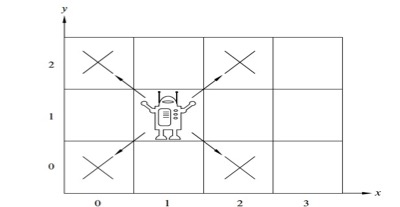
\includegraphics[width=3in]{robot-grid.png}
\end{center}
    
{\bf Theorem}: A robot on an infinite 2-dimensional integer grid starts at $(0,0)$ and at each step moves
to diagonally adjacent grid point. This robot can / cannot {\footnotesize({\it circle one})} reach $(1,0)$.


{\bf Definition} The set of positions the robot can visit  $P$ is defined by:
\[
\begin{array}{ll}
    \textrm{Basis Step: } & (0,0) \in P \\
    \textrm{Recursive Step: } & \textrm{If } (x,y) \in P  \textrm{, then } 
    \phantom{(x+1, y+1), (x+1, y-1), (x-1, y-1), (x-1, y+1)} \textrm{ are also in } P
\end{array}
\]

{\it Example elements of $P$ are}:
\vspace{40pt}

{\bf Lemma}: $\forall (x,y) \in P( (x+y \textrm{ is an even integer})~)$

{\it Why are we calling this a lemma?}


Proof of theorem using lemma: To show is $(1,0) \notin P$. Rewriting the lemma to explicitly 
restrict the domain of the universal, 
we have $\forall (x,y) ~(~ (x,y) \in P  \to (x+y \textrm{ is an even integer})~)$.  Since
the universal is true, 
$ (~ (1,0) \in P \to (1+0 \textrm{ is an even integer})~)$ is a true statement.
Evaluating the conclusion of this conditional statement: 
By definition of long division, since $1 = 0 \cdot 2 + 1$ (where $0 \in \mathbb{Z}$ and 
$1 \in \mathbb{Z}$ and $0 \leq 1 < 2$ mean that $0$ is the quotient and $1$ is the remainder), $1 ~\textrm{\bf mod}~ 2 = 1$ which is not $0$ 
so the conclusion is false.  A true conditional with a false conclusion must have a false hypothesis.
Thus, $(1,0) \notin P$, QED. $\square$

\vspace{20pt}

Proof of lemma by structural induction:

{\bf Basis Step}:

\vspace{100pt}


{\bf Recursive Step}:  Consider arbitrary $(x,y) \in P$.  To show is:
\[
(x+y \text{ is an even integer}) \to (\text{sum of coordinates of next position is even integer})
\]
Assume {\bf as the induction hypothesis, IH} that: 


\vspace{400pt} \newpage


The set $\mathbb{N}$ is recursively defined.
Therefore, the function $sumPow: \mathbb{N} \to \mathbb{N}$
which computes, for input $i$, the sum of the nonnegative powers of $2$
up to and including exponent $i$ is defined
recursively by

\begin{alignat*}{2}
    \text{Basis step:  } \qquad & sumPow(0) = 1 &\\
    \text{Recursive step:  } & \text{If } x \in \mathbb{N} \text{, then } &sumPow(x+1) = sumPow(x) + 2^{x+1}
\end{alignat*}

$sumPow(0) =$

\vspace{20pt}

$sumPow(1) =$

\vspace{20pt}

$sumPow(2) =$

\vspace{20pt}


Fill in the blanks in the following proof of 
\[
    \forall n \in \mathbb{N}~(sumPow(n) = 2^{n+1} - 1)
\]

{\bf Proof}: Since $\mathbb{N}$ is recursively defined, we proceed by \underline{\phantom{structural induction \hspace{0.3in}}}.

{\bf Basis case}: We need to show that \underline{\phantom{$sumPow(0) = 2^{0+1} - 1$ \hspace{0.2in}}}.
Evaluating each side: $LHS = sumPow(0) = 1$ by the basis case in the recursive definition
of $sumPow$; $RHS = 2^{0+1} - 1 = 2^1 - 1 = 2-1 = 1$. Since $1=1$, the equality holds.

{\bf Recursive case}: Consider arbitrary natural number $n$ and assume, as the 
\underline{\phantom{Induction Hypothesis (IH)}} that $sumPow(n) = 2^{n+1} - 1$. We need to show that
\underline{\phantom{$sumPow(n+1) = 2^{(n+1) + 1} - 1$}}.  Evaluating each side: 
\[
LHS = sumPow(n+1) \overset{\text{rec def}}{=} sumPow(n)  + 2^{n+1}\overset{\text{IH}}{=} (2^{n+1} - 1) + 2^{n+1}.
\]
\[
RHS = 2^{(n+1)+1}- 1 \overset{\text{exponent rules}}{=} 2 \cdot 2^{n+1} -1  = \left(2^{n+1} + 2^{n+1} \right) - 1
\overset{\text{regrouping}}{=}  (2^{n+1} - 1) + 2^{n+1} 
\]
Thus, $LHS = RHS$. The structural induction is complete and we have proved the universal generalization.
$\square$

 \vfill


\fbox{\parbox{\textwidth}{

{\bf Proof by Mathematical Induction}

To prove a universal quantification over the set of all integers greater than
or  equal to some  base integer $b$,

\vspace{-10pt}

\begin{itemize}
\item[] {\bf Basis Step}:  Show the property holds for $b$. 
\item[]  {\bf Recursive Step}:  Consider an arbitrary integer $n$ greater than or  equal to  $b$, assume
    (as the {\bf induction hypothesis})  that the property holds  for $n$, and use  this and
    other facts to  prove that  the property holds for $n+1$.
\end{itemize}

}} \newpage
\subsection*{Review}
\begin{enumerate}
\item \hspace{1in}\\ 

Recall the set $P$ defined by the recursive definition
\[
\begin{array}{ll}
    \textrm{Basis Step: } & (0,0) \in P\\
     \textrm{Recursive Step: } & \textrm{If } (x,y) \in P \textrm{ then } 
     (x+1, y+1) \in P \textrm{ and } (x+1, y-1) \in P \textrm{ and }\\ 
     & (x-1,y-1) \in P 
     \textrm{ and } (x-1, y+1) \in P
\end{array}
\]
\begin{enumerate}
\item Select all and only the ordered pairs below that are elements of $P$
\begin{enumerate}
\item $(0,0)$
\item $(4,0)$
\item $(1,1)$
\item $(1.5,2.5)$
\item $(0, -2)$
\end{enumerate}
\item What is another description of the set $P$ ? (Select all and only the true descriptions.)
\begin{enumerate}
\item $\mathbb{Z} \times \mathbb{Z}$
\item $\{ (n,n) ~|~ n \in \mathbb{Z} \}$
\item $\{ (a,b) \in \mathbb{Z} \times \mathbb{Z} ~|~ (a+b) \textbf{ mod } 2 =0 \}$
\end{enumerate}
\end{enumerate} \item \hspace{1in}\\ 

Select all and only the true statements below about the relationship between
structural induction and mathematical induction.
\begin{enumerate}
    \item Both structural induction and mathematical induction are proof strategies that 
    may be useful when proving universal claims about recursively defined sets.
    \item Mathematical induction is a special cae of structural induction, for the case when 
    the domain of quantification is $\{ n \in \mathbb{Z} \mid n \geq b\}$ for some integer $b$.
    \item Universal claims about the set of all integers may be proved using structural induction
    but not using mathematical induction.
\end{enumerate} \newpage
\item \hspace{1in}\\ 

Consider the following function definitions
\[
    2^n: \mathbb{N} \to \mathbb{N} \text{ given by } 2^0 = 1 ~~\text{ and }~~
    2^{n+1} = 2 \cdot 2^n  
\]
\[
    n!: \mathbb{N} \to \mathbb{N} \text{ given by } 0! = 1 ~~\text{ and }~~
    (n+1)! = (n+1) n!
\]
\begin{enumerate}
\item Select all and only true statements below: 
    \begin{enumerate}
        \item $2^0 < 0!$
        \item $2^1 < 1!$
        \item $2^2 < 2!$
        \item $2^3 < 3!$
        \item $2^4 < 4!$
        \item $2^5 < 5!$
        \item $2^6 < 6!$
        \item $2^7 < 7!$
    \end{enumerate}

\item Fill in the blanks in the following proof.

{\bf Claim}: For all integers $n$ greater than or equal to $4$, $2^n < n!$ \\

{\bf Proof}: We proceed by mathematical induction on the set of integers greater than or equal to $4$.

{\bf Basis step}: Using the \underline{\hspace{0.2in}BLANK 1\hspace{0.2in}}, 
\[
    2^4 = 2 \cdot 2^3 = 2 \cdot 2 \cdot 2^2 = 2 \cdot 2 \cdot 2 \cdot 2^1 =
    2 \cdot 2 \cdot 2 \cdot 2 \cdot 2^0 =
    2 \cdot 2 \cdot 2 \cdot 2 \cdot 1 = 16 
\]
and
\[
    4! = 4 \cdot 3! = 4 \cdot 3 \cdot 2! 
    = 4 \cdot 3 \cdot 2 \cdot 1! = 4 \cdot 3 \cdot 2 \cdot 1 \cdot 0!
    = 4 \cdot 3 \cdot 2 \cdot 1 \cdot 1 = 24
\]
Since $16 < 24$, we have proved that $2^4 < 4!$~, as required.\\

{\bf Recursive step}: Consider an arbitrary integer $k$ that 
is greater than or equal to $4$
and assume as the \underline{\hspace{0.2in}BLANK 2\hspace{0.2in}}, 
that $2^k < k!$~. We want to show that $2^{k+1} < (k+1)!$~.
\begin{align*}
    2^{k+1} &= 2 \cdot 2^{k} \qquad \text{by }\underline{\hspace{0.2in}BLANK 3\hspace{0.2in}}\\
        &< 2 \cdot k! \qquad \text{by }\underline{\hspace{0.2in}BLANK 4\hspace{0.2in}}\\
        &< k \cdot k! \qquad \text{by }\underline{\hspace{0.2in}BLANK 5\hspace{0.2in}}\\
        &< (k+1) \cdot k!  \qquad \text{by }\underline{\hspace{0.2in}BLANK 6\hspace{0.2in}}\\
        &= (k+1)!  \qquad \text{by }\underline{\hspace{0.2in}BLANK 7\hspace{0.2in}}\\
\end{align*}
as required.

\begin{enumerate}
    \item properties of addition, multiplication, and $<$ for real numbers
    \item definitions of the functions $2^n$ and $n!$
    \item definition of $k$
    \item induction hypothesis
\end{enumerate}
\end{enumerate} \end{enumerate}

\newpage
\section*{Friday November 5}


{\bf Definition} The set of linked lists of natural numbers $L$ is defined recursively by
\[
\begin{array}{ll}
    \textrm{Basis Step: } & [] \in L \\
    \textrm{Recursive Step: } & \textrm{If } l \in L\textrm{ and }n \in \mathbb{N} \textrm{, then } (n, l) \in L
\end{array}
\] 

Visually:

\vspace{50pt}

Example: the list with two nodes whose first node has $20$ and whose second node
has $42$

\vspace{50pt} 

{\bf Definition}: The length of a linked list of natural numbers $L$, $length: L \to \mathbb{N}$ is defined by
\[
\begin{array}{llll}
\textrm{Basis Step:} &  & length(~[]~) &= 0 \\
\textrm{Recursive Step:} & \textrm{If } l \in L\textrm{ and }n \in \mathbb{N}\textrm{, then  } & length(~(n, l)~)  &= 1+ length(l)
\end{array}
\]
 \vspace{50pt}


{\bf Definition}: The function $prepend : L \times \mathbb{N} \to L$ that adds an element at the 
front of a linked list is defined by
\[
\phantom{prepend(~(l, n)~) = (n, l)}
\]
 \vspace{50pt}


{\bf Definition} The function $append : L \times \mathbb{N} \to L$ that 
adds an element at the end of a linked list is defined by
\[
\begin{array}{llll}
\textrm{Basis Step:} & \textrm{If } m \in \mathbb{N}\textrm{ then } & \phantom{append(~([], m)~)} & \phantom{= (m, []) }\\
\textrm{Recursive Step:} & \textrm{If } l \in L\textrm{ and }n \in \mathbb{N}\textrm{ and }m \in \mathbb{N}\textrm{, then  } & \phantom{append(~(~(n, l), m~)~) } &\phantom{= (n, append(~(l, m)~)~)}
\end{array}
\] \vspace{50pt}
\newpage


{\bf Claim}: $\forall l \in L ~ (~length(~append(~(l, 100)~)~) > length(l)~)$

{\bf Proof:} By structural induction on $L$, we have two cases:

{\bf Basis Step}

    \begin{tabular}{l p{3.5in}}
     1. \textbf{To Show} $length(~append(~([], 100)~)~) > length(~[]~)$
    & Because $[]$ is the only element defined in the basis step of $L$, 
    we only need to prove that the property holds for $[]$.\\
    &  \\
     2. \textbf{To Show} $length(~(100,[])~) > length(~[]~)$
    &  By basis step in definition of $append$.\\
    &  \\
     3. \textbf{To Show} $(1 +length(~[]~)) > length(~[]~)$
    &  By recursive step in definition of $length$.\\
    &  \\    
     4. \textbf{To Show} $1+0 > 0$
    &  By basis step in definition of $length$.\\
    &  \\    
    5. $T$
    & By properties of integers \\
    &  \\    
    QED & Because we got to $T$ only by rewriting \textbf{To Show} to equivalent statements, using well-defined proof techniques, and applying definitions. \\
    \end{tabular}

{\bf Recursive Step}

Consider an arbitrary: $l' \in L$, $n \in \mathbb{N}$, and we  assume
as the {\bf induction hypothesis} that:
\[
length(~append(~(l', 100~)~)~) > length(l')
\]
Our goal is to show that $length(~append( ~(~(n,l'), 100~)~)~) > length(~(n,l')~)$ is also true. 
We start by working with
one side of the candidate inequality:
\begin{align*}
LHS &= length(~append( ~(~ (n,l'), 100~)~)~) \\
&= length(~(n, append(~(l', 100)~)~ )~) \qquad \text{by the recursive definition of $append$}\\
&= 1 + length(~ append(~(l', 100)~) ~) \qquad \text{by the recursive definition of $length$}\\
&> 1+ length(l')  \qquad \text{by the induction hypothesis}\\
&= length( (n,l') )  \qquad \text{by the recursive definition of $length$}\\
&= RHS 
\end{align*} \newpage


Prove or disprove: $\forall n \in \mathbb{N} ~\exists l \in L ~(~length(l) = n~)$

\vspace{300pt} \newpage
\subsection*{Review}


Recall the definition of linked lists from class.

Consider this (incomplete) definition:

{\bf Definition} The function $\textit{increment} : \underline{\hspace{6em}}$ 
that adds 1 to the data in each node of a linked list is defined by:
\[
\begin{array}{llll}
& & \textit{increment} : \underline{\hspace{3em}} & \to \underline{\hspace{3em}} \\
\textrm{Basis Step:} & & \textit{increment}([]) & = [] \\
\textrm{Recursive Step:} & \textrm{If } l \in L, n \in \mathbb{N} & \textit{increment}((n, l)) & = (1 + n, \textit{increment}(l))
\end{array}
\]

Consider this (incomplete) definition:

{\bf Definition} The function $\textit{sum} : L \to \mathbb{N}$ that adds 
together all the data in nodes of the list is defined by:
\[
\begin{array}{llll}
& & \textit{sum} : L & \to \mathbb{N} \\
\textrm{Basis Step:} & & \textit{sum}([]) & = 0 \\
\textrm{Recursive Step:} & \textrm{If } l \in L, n \in \mathbb{N} & \textit{sum}((n, l)) & = \underline{\hspace{8em}}
\end{array}
\]

You will compute a sample function application and then fill in the 
blanks for the domain and codomain of each of these functions.

\begin{enumerate}
    \item Based on the definition, what is the result of $\textit{increment}((4, (2, (7, []))))$? Write your answer directly with no spaces.
    
    \item Which of the following describes the domain and codomain of \textit{increment}?
    
    \begin{multicols}{2}
    \begin{enumerate}
        \item The domain is $L$ and the codomain is $\mathbb{N}$
        \item The domain is $L$ and the codomain is $\mathbb{N} \times L$
        \item The domain is $L \times \mathbb{N}$ and the codomain is $L$
        \item The domain is $L \times \mathbb{N}$ and the codomain is $\mathbb{N}$
        \item The domain is $L$ and the codomain is $L$
        \item None of the above
    \end{enumerate}
    \end{multicols}
    
    \item Assuming we would like $sum((5, (6, [])))$ to evaluate to $11$ and $sum((3, (1, (8, []))))$ to evaluate to $12$, which of the following could be used to fill in the definition of the recursive case of \textit{sum}?
    
     \begin{multicols}{2}
    \begin{enumerate}
        \item $\begin{cases}
            1 + \textit{sum}(l) & \textrm{when } n \neq 0 \\
            \textit{sum}(l) & \textrm{when } n = 0 \\
        \end{cases}$
        \item $1 + \textit{sum}(l)$
        \item $n + \textit{increment}(l)$
        \item $n + \textit{sum}(l)$
        \item None of the above
    \end{enumerate}
    \end{multicols}
    
    \newpage
    \item Choose only and all of the following statements that are \textbf{well-defined}; that is, they correctly reflect the domains and codomains of the functions and quantifiers, and respect the notational conventions we use in this class. Note that a well-defined statement may be true or false.

    \begin{multicols}{2}    
    \begin{enumerate}
        \item $\forall l \in L \, (\textit{sum}(l))$
        \item $\exists l \in L \, (\textit{sum}(l) \land \textit{length}(l))$
        \item $\forall l \in L \, (\textit{sum}(\textit{increment}(l)) = 10)$
        \item $\exists l \in L \, (\textit{sum}(\textit{increment}(l)) = 10)$
        \item $\forall l \in L \, \forall n \in \mathbb{N} \, ((n \times l) \subseteq L)$
        \item $\forall l_1 \in L \, \exists l_2 \in L \, (\textit{increment}(\textit{sum}(l_1)) = l_2)$
        \item $\forall l \in L \, (\textit{length}(\textit{increment}(l)) = \textit{length}(l))$
    \end{enumerate}
    \end{multicols}
    
    \item Choose only and all of the statements in the previous part that are both well-defined and true.
\end{enumerate} 
\end{document}
